\documentclass{article}[a4paper, oneside, 11pt]

\usepackage[T1]{fontenc}
\usepackage[utf8]{inputenc}
\usepackage{calc}
\usepackage{amsmath, amssymb, amsthm, thmtools, amsfonts}
\usepackage{mathtools}
\usepackage[nochapters,pdfspacing]{classicthesis}
%\usepackage{hyperref}% clashes with classicthesis
\usepackage{cleveref}
\usepackage[siunitx]{circuitikz}
\usepackage{booktabs}
\usepackage{graphicx}
\usepackage{caption}
\usepackage{subcaption}
\usepackage{geometry}
\usepackage{float}
\usepackage{mdframed}
\usepackage{xcolor}
\usepackage{siunitx}
\usepackage[italian]{babel}
\usepackage{pgfplots}
\usepackage{titling}
\usepackage{listings}
\usepackage{lmodern}
\usepackage{url}
\usepgfplotslibrary{external} 
\tikzexternalize

\pgfplotsset{compat=1.15}
\lstset{
language=Python,
basicstyle=\ttfamily,
columns=fullflexible,
keepspaces=true,
}
\mdfsetup{linewidth=0.6pt}
\graphicspath{{./figs/}}
\makeatletter
\def\input@path{{./figs/}}
%or: \def\input@path{{/path/to/folder/}{/path/to/other/folder/}}
\makeatother

% Default fixed font does not support bold face
\DeclareFixedFont{\ttb}{T1}{txtt}{bx}{n}{12} % for bold
\DeclareFixedFont{\ttm}{T1}{txtt}{m}{n}{12}  % for normal

% Custom colors
\usepackage{color}
\definecolor{deepblue}{rgb}{0,0,0.5}
\definecolor{deepred}{rgb}{0.6,0,0}
\definecolor{deepgreen}{rgb}{0,0.5,0}

% Commands 
\newcommand{\executeiffilenewer}[3]{%
	\ifnum\pdfstrcmp{\pdffilemoddate{#1}}%
		{\pdffilemoddate{#2}}>0%
	{\immediate\write18{#3}}\fi%
}
% input .svg --> .pdf_tex graphs
\newcommand{\includesvg}[1]{%
	\executeiffilenewer{#1.svg}{#1.pdf}%
	{inkscape -z -D --file=#1.svg %
	--export-pdf=#1.pdf --export-latex}%
	\input{#1.pdf_tex}%
}

\newcommand{\eps}{\varepsilon}
\renewcommand{\phi}{\varphi}
\newcommand{\loc}{\mathit{loc}}
\newcommand{\weakto}{\rightharpoonup}
\newcommand{\implied}{\Longleftarrow}
\let\subsetstrict\subset
\renewcommand{\subset}{\subseteq}
\renewcommand{\supset}{\supseteq}

% calligraphic letters
\newcommand{\A}{\mathcal A}
\newcommand{\B}{\mathcal B}
\newcommand{\C}{\mathcal C}
\newcommand{\D}{\mathcal D}
\newcommand{\E}{\mathcal E}
\newcommand{\F}{\mathcal F}
\newcommand{\FL}{\mathcal F\!\mathcal L}
\renewcommand{\H}{\mathcal H}
\newcommand{\K}{\mathcal K}
\renewcommand{\L}{\mathcal L}
\newcommand{\M}{\mathcal M}
\renewcommand{\P}{\mathcal P}
\renewcommand{\S}{\mathcal S}
\newcommand{\U}{\mathcal U} %% intorni

% blackboard letters
\newcommand{\CC}{\mathbb C}
\newcommand{\HH}{\mathbb H}
\newcommand{\KK}{\mathbb K}
\newcommand{\NN}{\mathbb N}
\newcommand{\QQ}{\mathbb Q}
\newcommand{\RR}{\mathbb R}
\newcommand{\TT}{\mathbb T}
\newcommand{\ZZ}{\mathbb Z}

%\newcommand{\abs}[1]{{\left|#1\right|}}
\newcommand{\Abs}[1]{{\left\Vert #1\right\Vert}}
\newcommand{\enclose}[1]{{\left( #1 \right)}}
\newcommand{\Enclose}[1]{{\left[ #1 \right]}}
\newcommand{\floor}[1]{\left\lfloor #1 \right\rfloor}
\newcommand{\ceil}[1]{\left\lceil #1 \right\rceil}

\newcommand{\To}{\rightrightarrows}
\renewcommand{\vec}[1]{\boldsymbol #1}
\newcommand{\defeq}{:=}
\DeclareMathOperator{\divergence}{div}
\renewcommand{\div}{\divergence}
\DeclareMathOperator{\Imaginarypart}{Im}
\renewcommand{\Im}{\Imaginarypart}
\DeclareMathOperator{\Realpart}{Re}
\renewcommand{\Re}{\Realpart}
%\DeclareMathOperator{\arg}{arg}
\DeclareMathOperator{\tg}{tg}
\DeclareMathOperator{\arctg}{arctg}
\DeclareMathOperator{\settsinh}{settsinh}
\DeclareMathOperator{\settcosh}{settcosh}
\DeclareMathOperator{\tr}{tr}
\DeclareMathOperator{\im}{im}
\DeclareMathOperator{\sgn}{sgn}
\DeclareMathOperator{\diag}{diag}

\declaretheoremstyle[
spaceabove=6pt, spacebelow=6pt,
headfont=\normalfont\bfseries\itshape,
notefont=\mdseries, notebraces={(}{)},
bodyfont=\normalfont,
postheadspace=1em,
qed=,
%shaded={rulecolor=pink!30,rulewidth=1pt,bgcolor=pink!10}
]{exercise_style}

\declaretheoremstyle[
spaceabove=6pt, spacebelow=6pt,
postheadspace=1em,
qed=,
%shaded={rulecolor=blue!20,rulewidth=1pt,bgcolor=blue!5}
]{theorem_style}

\declaretheoremstyle[
spaceabove=6pt, spacebelow=6pt,
postheadspace=1em,
qed=,
%shaded={rulecolor=yellow!50,rulewidth=1pt,bgcolor=yellow!5}
]{axiom_style}

\declaretheorem[name=Teorema]{theorem}
\declaretheorem[name=Lemma,sibling=theorem]{lemma}
\declaretheorem[name=Proposizione,sibling=theorem]{proposition}
\declaretheorem[name=Corollario,sibling=theorem]{corollary}
\declaretheorem[name=Paradosso,sibling=theorem]{paradox}
\declaretheorem[style=axiom_style,name=Assioma,sibling=theorem]{axiom}
\declaretheorem[name=Definizione,sibling=theorem]{definition}
\declaretheorem[style=exercise_style,name=Esempio,sibling=theorem]{example}
\declaretheorem[style=exercise_style,name=Esercizio,sibling=theorem]{exercise}
\declaretheorem[style=exercise_style,name=Osservazione,sibling=theorem]{remark}

% Logarithm with arbitrary base.
% -> log_10
\newcommand{\llog}[1][10]{\log_{#1}}

% Absolute value.
% -> |x|
\newcommand{\abs}[1]{\left| #1 \right|}

% Powers.
% -> x^a
\newcommand{\power}[2][2]{\left( #2 \right)^{#1}}

% Square.
% -> x^2
\newcommand{\sq}[1]{\power[2]{#1}}

% Expansion of the binomial coefficient.
% -> n1!/(n2!(n1 - n2)!)
\newcommand{\binomexpr}[2]{\frac{#1!}{#2!(#1 - #2)!}}

% Expression evaluation at a given point with square brackets.
% -> [x]_{a}
\newcommand{\at}[2]{\left[ #1\right]_{\makebox[-1pt][l]{${\scriptstyle#2}$}}}

% Expression evaluation in an interval.
% -> [x] _{a}^{b}
\newcommand{\eval}[3]{\left.#1%
  \right|_{\makebox[-1pt][l]{${\scriptstyle#2}$}}^{\makebox[-1pt][l]{${\scriptstyle#3}$}}}

% Upright d in math mode (for differentials).
% -> d
\newcommand{\ud}{\mathrm{d}}

% Differential.
% -> dx
\newcommand{\diff}[1][x]{\,\ud{#1}}

% Base command for defining derivatives.
% -> df/dx or d^kf/dx^k
\newcommand{\basederivative}[4][]{%
  \displaystyle%
  \ifx\\#1\\\frac{#4#2}{#4#3}%
  \else%
  \frac{#4^#1#2}{#4#3^#1}%
  \fi%
}

% Total derivative.
% -> df/dx(x) or d^kf/dx^k(x)
\newcommand{\td}[4][]{%
  \basederivative[#1]{#2}{#3}{\ud}%
  \ifx\\#4\\%
  \else%
  \mkern-4mu\left(#4\right)%
  \fi%
}

% Partial derivative.
% -> df/dx(x) or d^kf/dx^k(x)
\newcommand{\pd}[4][]{%
  \basederivative[#1]{#2}{#3}{\partial}%
  \ifx\\#4\\%
  \else%
  \mkern-4mu\left(#4\right)%
  \fi%
}

\newcommand{\intinf}{\int_{-\infty}^{\infty}\!\!\!}

\newcommand{\cinterval}[2]{\left[\, #1,~#2 \,\right]}

\newcommand{\linterval}[2]{\left[\, #1,~#2 \,\right)}

\newcommand{\rinterval}[2]{\left(\, #1,~#2 \,\right]}

\newcommand{\ointerval}[2]{\left(\, #1,~#2 \,\right)}

\newcommand{\prob}[1]{\displaystyle P\left(#1\right)}

\newcommand{\pvalue}{\emph{$p$-value}}

\newcommand{\cond}{\,|\,}

\newcommand{\expect}[1]{\displaystyle E\left[#1\right]}

\newcommand{\mom}[2][]{\displaystyle {\cal M}_{#2}\ifx\\#1\\\else(#1)\fi}

\newcommand{\momalg}[1]{\displaystyle \lambda_{#1}}

\newcommand{\momcen}[1]{\displaystyle \mu_{#1}}

\newcommand{\skewness}{\displaystyle \gamma_1}

\newcommand{\kurtosis}{\displaystyle \gamma_2}

\newcommand{\charf}[1][x]{\phi_{#1}}

\newcommand{\momgenf}[1][x]{M_{#1}}

\newcommand{\fwhm}{{\scriptstyle \textsc{FWHM}}}

\newcommand{\hwhm}{{\scriptstyle \textsc{HWHM}}}

\newcommand{\median}{\mu_{\nicefrac{1}{2}}}

\newcommand{\var}[1]{\ensuremath{\text{Var}\left(#1\right)}}

\newcommand{\cov}[2]{\ensuremath{\text{Cov}\left(#1, #2\right)}}

\newcommand{\corr}[2]{\ensuremath{\text{Corr}\left(#1, #2\right)}}

\newcommand{\like}{\mathcal L}

\newcommand{\likelihood}[2][]{\like\ifx\\#2\\\else(#2\ifx\\#1\\\else;#1\fi)\fi}

\newcommand{\chisq}{\ensuremath{\chi^2}}

\newcommand{\chisquare}[2][]{\chisq\ifx\\#2\\\else(#2\ifx\\#1\\\else;#1\fi)\fi}

\newcommand{\loglikelihood}[2][]{\log\likelihood[#1]{#2}}

\newcommand{\pdf}[3][]{#2(#3\ifx\\#1\\\else;#1\fi)}

\newcommand{\binomialpdf}[2][]{\pdf[#1]{\mathcal B}{#2}}

\newcommand{\multinomialpdf}[2][]{\pdf[#1]{\mathcal M}{#2}}

\newcommand{\poissonpdf}[2][]{\pdf[#1]{\mathcal P}{#2}}

\newcommand{\uniformpdf}[2][]{\pdf[#1]{u}{#2}}

\newcommand{\exponentialpdf}[2][]{\pdf[#1]{\varepsilon}{#2}}

\newcommand{\gausspdf}[2][]{\pdf[#1]{N}{#2}}

\newcommand{\chisquarepdf}[2][]{\pdf[#1]{\wp}{#2}}

\newcommand{\cauchypdf}[2][]{\pdf[#1]{c}{#2}}

\newcommand{\erf}[1]{\ensuremath{\text{erf}\left(#1\right)}}

\newcommand{\dccases}[4][]{#2 \ifx\\#2\\\else=\fi %
  \begin{cases}
    \displaystyle #3 & \text{per variabili discrete}\\
    \displaystyle #4 & \text{per variabili continue}#1
  \end{cases}
}
\newcommand\Scaleforall[1]{\vcenter{\hbox{\scalefont{#1}$\forall$}}}

\DeclareMathOperator*\forevery{%
  \vphantom\sum
  \mathchoice{\Scaleforall{2}}{\Scaleforall{1.4}}{\Scaleforall{1}}{\Scaleforall{0.75}}}
 
 % Default fixed font does not support bold face
\DeclareFixedFont{\ttb}{T1}{txtt}{bx}{n}{12} % for bold
\DeclareFixedFont{\ttm}{T1}{txtt}{m}{n}{12}  % for normal

% Custom colors
\usepackage{color}
\definecolor{deepblue}{rgb}{0,0,0.5}
\definecolor{deepred}{rgb}{0.6,0,0}
\definecolor{deepgreen}{rgb}{0,0.5,0}

\geometry{a4paper, left=25mm, right=25mm, top=25mm, bottom=25mm}
\title{Modellizzazione della resistenza di diodi a giunzione PN per alte 
correnti di lavoro}
\author{L.~Ciucci(\thanks{Dipartimento di Fisica E.~Fermi, Universit\`a di Pisa 
- Pisa, Italy} )~\and S.~Bruzzesi(\protect\footnotemark[1] )~\and 
M.~Romagnoli(\protect\footnotemark[1] )~\and 
M.~Alighieri(\protect\footnotemark[1] )~\and 
B.~Tomelleri(\protect\footnotemark[1] )}
%\date{2020/11/01}

\begin{document}
\maketitle

%================================================================
%                            Riassunto
%================================================================
\begin{mdframed}
\textbf{Riassunto:} --- Si è studiato il comportamento di un diodo in silicio
PN, ricostruendone sperimentalmente la curva caratteristica $V-I$, al fine di
mettere in risalto la sua componente resistiva. A questo scopo è stata
esplorata un'ampia zona della curva, in particolar modo per alti valori di
$I$, dove questa caratteristica è maggiormente apprezzabile. Proponiamo dunque
un'estensione della legge di Shockley, tramite l'aggiunta di un termine
resistivo, in grado di descrivere l'elemento -ohmico- della giunzione.
%;il che equivale a modellare un diodo reale come un resistore in serie
%ad un diodo ideale.
La nuova curva caratteristica prevede un andamento sempre più lineare di $I$
al crescere di $V$ e questo risulta in accordo con l'andamento dei dati
sperimentali.
\\\\
PACS 01.40.-d – Education.\\
PACS 01.50.Pa – Laboratory experiments and apparatus.
\end{mdframed}


%================================================================
%                         Introduzione
%================================================================
\section{Introduzione}
La limitata conducibilità intrinseca al silicio, di cui è composta la
giunzione bipolare, comporta la presenza di una sua componente resistiva:
per effetti termico-dissipativi questa ha un effetto sempre meno
trascurabile, all'aumentare della tensione ai suoi capi, sul passaggio di
corrente attraverso il diodo.
Per poter descrivere la parte resistiva di un diodo percorso da correnti
di alta intensità %\footnote{Nel nostro caso per un diodo 1N4007 la massima
%intensità di corrente continua $I_F = 1.0$ A nominali.}
si propone un modello semplice, di resistenza parassita in serie, verificandone
l'accordo con i risultati sperimentali su un'ampia regione di punti di lavoro.

%================================================================
%                         Cenni teorici
%================================================================
\section{Cenni Teorici}
Secondo le nostre ipotesi, un diodo reale può essere schematizzato come un
resistore ohmico %\footnote{Vista la simmetria della giunzione, propriamente
%si considerano due resistori -equivalenti- disposti ai lati del diodo ideale,
%la cui resistenza non è indipendente dalle condizioni di operazione.}
ed un diodo ideale in serie. Pertanto ci aspettiamo che la corrente che
attraversa questi elementi del circuito sia la stessa:
\begin{equation}
	I = \frac{\Delta V_{\text{resistore}}}{R} =
	I_0 \left( e^{\frac{\Delta V_{\text{diodo}}}{\eta V_t}} - 1\right)
\end{equation}
Dunque la relazione che lega la corrente alla tensione ai capi del diodo può 
essere espressa secondo la legge:
\begin{equation}\label{eq: model}
	\Delta V = \Delta V_{\text{diodo}} + \Delta V_{\text{resistore}} =
	\eta V_T \ln{\left(\frac{I+I_0}{I_0}\right)} + RI
\end{equation}
\begin{figure}[!ht]
	\centering 
 		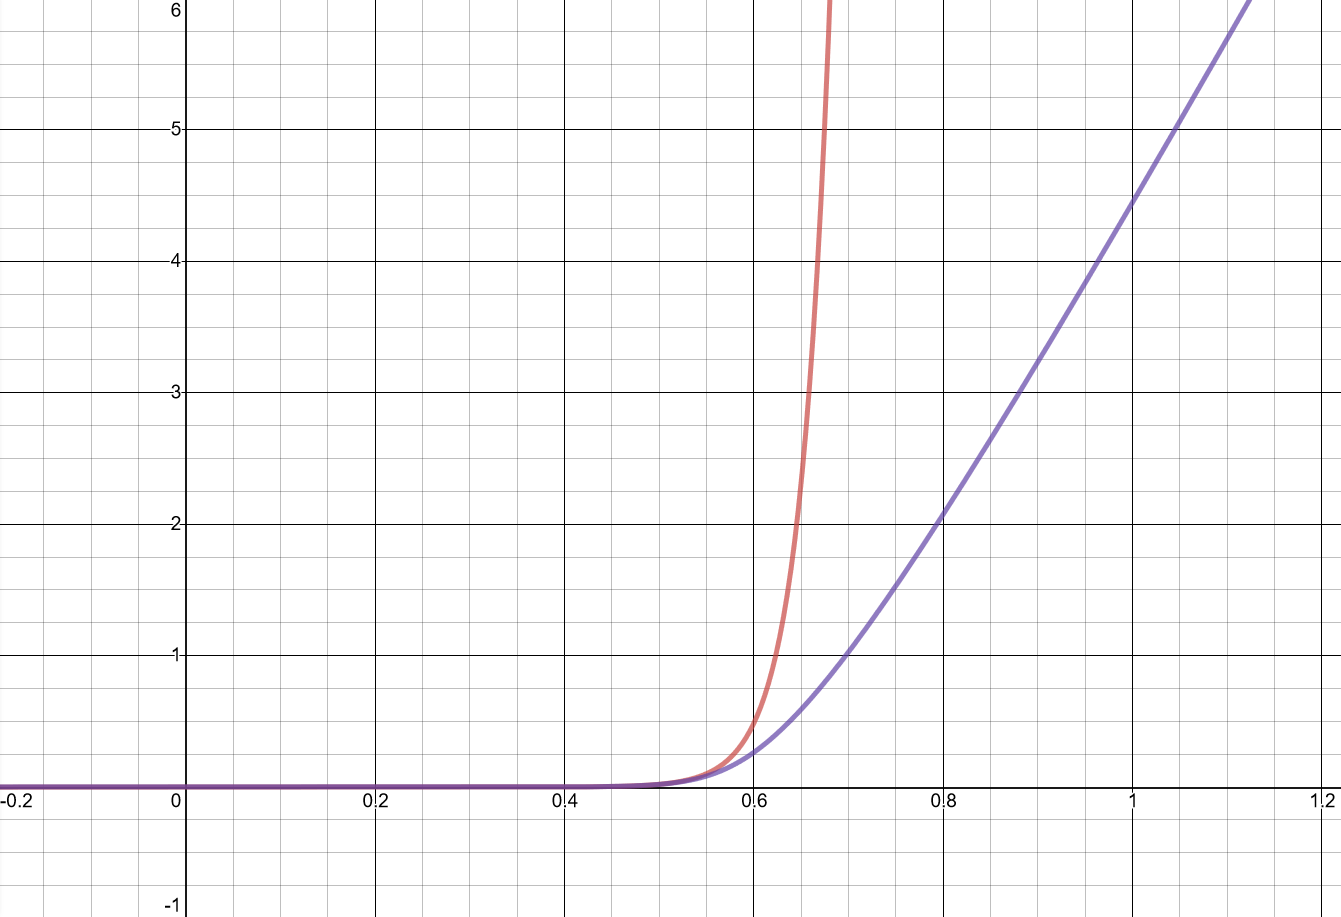
\includegraphics[scale=0.25]{confronto_curve.png}
 	\caption{confronto degli andamenti: la curva di Shockley (in rosso) e la 
	legge \eqref{eq: model} (in viola)}
\end{figure}

%================================================================
%                Metodo e apparato sperimentale
%================================================================
\section{Metodo e apparato sperimentale}
Onde evitare sostanziali aumenti di temperatura, oltre ad eventuali danni
a questi stessi, si imprimono correnti impulsate sul circuito. 
%e le conseguenti variazioni di resistenza nei componenti 
La durata degli impulsi è inferiore ai 200 $\mu$s, che corrisponde ad
un'energia impressa inferiore a 1 mJ (dunque ad un aumento della temperatura
del semiconduttore inferiore a 0.5 K).
%Dovendo lavorare con correnti relativamente alte per il circuito sotto studio,
%al fine di minimizzare effetti termici-dissipativi secondari ed evitare danni
%all'apparato, si imprimono sui componenti correnti pulsate o di durate molto
%brevi, limitando dunque il trasferimento di energia sui componenti.

%================================
%           Apparato
%================================
\subsection{Apparato}
L'apparato sperimentale è costituito da un circuito, realizzato su basetta 
sperimentale (\emph{breadboard}), il cui scopo è generare le correnti
impulsate appena descritte attraverso il diodo $D1$ e la resistenza $R1$.
La misura della differenza di potenziale agli estremi della $R_1$ permette
di stimare la corrente che circola sul diodo.
% Per poter esplorare una larga banda di punti di lavoro del diodo,
Per poter esplorare una larga banda di correnti di lavoro
% Forse meglio una larga fascia di correnti, visto che il compito della
% resistenza è proprio quello di limitare la corrente sul diodo?
si è variata opportunamente la resistenza in serie al diodo, scegliendo tra
le seguenti:
\begin{table}[H]% la tabella deve stare per forza sotto "seguenti:"
    \begin{center}
	\begin{tabular}{lll}
	    \toprule
	    $R1$ nom. [$\Omega$] & $R1$ mult. [$\Omega$] \\ 
	    \midrule
	    \midrule
	    $0.22 \pm 3 \% $         	& $0.226 \pm 0.008$ \\
	    $2.2 \pm 5 \% $          	& $2.212 \pm 0.008$ \\
	    $22 \pm 5 \% $           	& $21.86 \pm 0.010$ \\ 
		$220 \pm 5 \% $          	& $216.22 \pm 0.07$ \\
	    $2.2\; \rm k \pm 5 \% $       & $2202.1 \pm 0.4$ \\
	    $22\; \rm k \pm 5 \% $       & ($21.7 \pm 0.3)10^3$ \\
	    $0.22\; \rm M \pm 5 \% $      & ($217 \pm 3)10^3$ \\
	    \bottomrule
	\end{tabular}
	\caption{I valori delle resistenze poste in serie al diodo, riportate in
		valore nominale e misurate con multimetro digitale. \label{tab:res}}
    \end{center}
\end{table}
Peruna descrizione del metodo di misurazione delle resistenze si rimanda a
\nameref{app: A}.
D'altra parte, per fornire una tensione regolabile e sufficientemente stabile
durante un impulso, nel circuito si impiega il condensatore $C1$, la cui
tensione, carica e scarica sono controllate dalla maglia destra del circuito.
Nel circuito si distingue inoltre la maglia che si occupa di collegare, sotto
istruzione di un microcontrollore, il condensatore alla serie $R1-D1$
attraverso un MOS-FET.\\
Il circuito è alimentato da 2 tensioni continue, fornite da un alimentatore
stabilizzato switching e da un Buck Boost Converter.
%,alle maglie di "carica/scarica" e di "switch" rispettivamente
Un segnale fornito su $T2$ provoca la carica del condensatore mentre su $T3$
la sua scarica. Un segnale (invertito) su $T1$ innesca l'impulso di corrente
sul diodo.\\
La tensione di C$1$ è misurata attraverso un partitore di tensione collegato 
ad \verb+OUT3+ ed alla scheda di controllo, mentre la d.d.p. tra i punti
\verb+OUT1+ e \verb+OUT2+ è misurata direttamente.\\
Come MCU per la gestione dell'apparato si è scelta la scheda 
\verb+Teensy 3.2+\cite{teensy}. Questa si occupa del controllo dei segnali e 
delle letture analogiche. In particolare \verb+Teensy+ permette la lettura
analogica sincronizzata differenziale veloce, essendo dotato di due ADC,
entrambi con una risoluzione reale di 12 bit. La lettura differenziale è
fondamentale per acquisire coppie di dati per le tensioni ai capi del diodo
e della resistenza.

\begin{figure}[!htb]
	\centering 
 		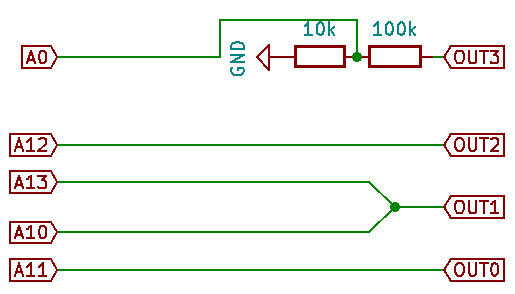
\includegraphics[scale=0.5]{./measure.png}
 	\caption{Schema circuitale del sistema di lettura (verso\texttt{Teensy})
	\label{sch:rdng}}
\end{figure}

\begin{figure}[h!t]% so che è brutto che lascia un po' di spazio bianco ma altrimenti lo metterebbe dentro calibrazione
	\centering 
 		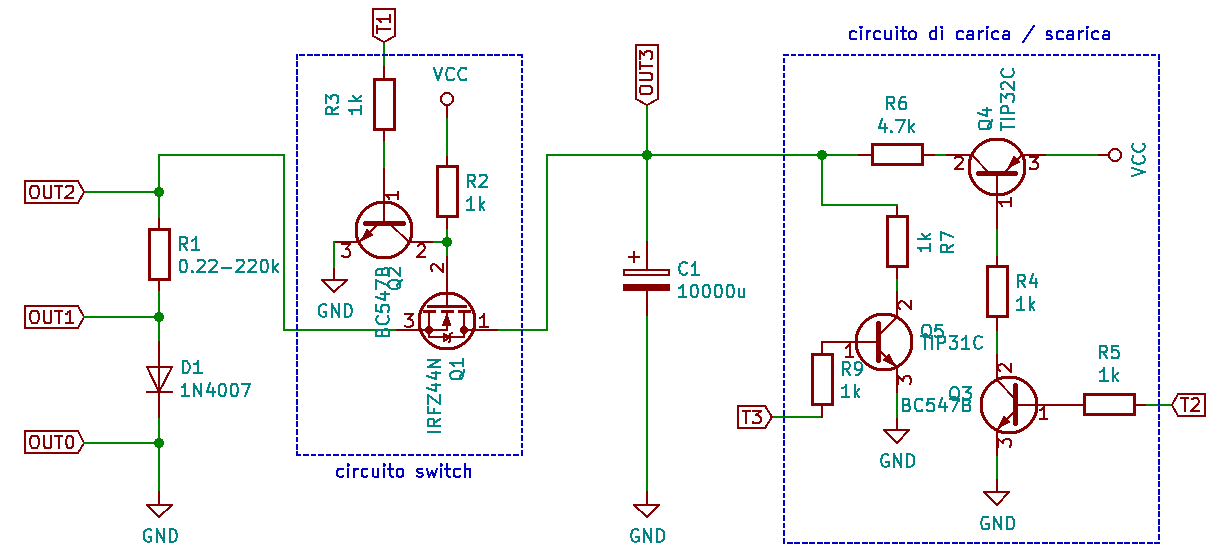
\includegraphics[scale=0.5]{./gestione.png}
 	\caption{Circuito globale per la gestione del diodo \label{sch:gest}}
\end{figure}

%===============================
%         Calibrazione
%================================
\subsection{Calibrazione}\label{sec: cal}

La calibrazione dei canali \verb+ADC0+ e \verb+ADC1+ è stata effettuata
basandosi sulle letture differenziali, rispettivamente fra i pin \verb+A10+
e \verb+A11+; fra \verb+A12+ e \verb+A13+. E’ stata calibrata la lettura
di ciascuna delle due coppie separatamente.

I pin volti alla lettura della tensione maggiore sono stati collegati al 
centrale di un potenziometro, a sua volta collegato ad un generatore di 
potenziale con tensione in ingresso pari a 3.3V . Gli altri due pin sono stati 
invece collegati a massa.

Variando la resistenza e, conseguentemente, la differenza di potenziale in 
ingresso, è stato possibile calcolare media, deviazione standard campione
e deviazione standard della media relative a ciascuna tensione per 
un gruppo di 10000 misure effettuate con \verb+Teensy+ (si veda il 
\href{https://github.com/LucaCiucci/relaz_seme/blob/master/sketches/teensy_calib/teensy_calib.ino}{relativo sketch}).
Il centrale del potenziometro e la massa sono state, inoltre, collegate ad un
multimetro digitale, in modo da poter associare la tensione misurata in
Volt alla corrispondente lettura digitalizzata dal MCU. Abbiamo assunto come
incertezze sulle misure i valori dichiarati nelle specifiche del multimetro,
mentre come errori sulle letture digitali abbiamo preso le deviazioni standard
dalla media.

Dopodiché le misure relative a ciascuna coppia di boccole sono state poste 
all’interno di un grafico con i dati raccolti da \verb+Teensy+ sulle ascisse
e i valori misurati col multimetro sulle ordinate. Dunque si è effettuato un
fit lineare attraverso la legge:
\begin{equation}
y(x; m, q)  = m x + q
\end{equation}

lasciando liberi entrambi i parametri $m$ e $q$. Riportiamo sotto i parametri
di best-fit relativi ad \verb+ADC0+ ed \verb+ADC1+ e le rispettive covarianze:
% Forse le varianze sono superflue? Il lettore le può ottenere semplicemente
% quadrando le incertezze sui parametri.
% Solitamente le covarianze si riportano normalizzate, così risultano poco
% immediate come indice di correlazione fra i parametri.
\begin{align*}
	&\qquad \texttt{ADC0}	&&\qquad  \texttt{ADC1} \\
	m_0 &= 0.7968 \pm  0.0033  \; \mathrm{mV/digit} 
	& m_1  &= 0.7954 \pm 0.0026  \; \mathrm{mV/digit} \\
	q_0 &= - 0.18 \pm 0.34  \; \mathrm{mV} 	
	&q_1 &= 3.84  \pm 0.26  \; \mathrm{mV} \\
	%\var{m_0}  &= 1.1 \cdot 10^{-11}  \; \mathrm{V}^2 /\mathrm{digit}^2
	%&\var{m_1} &= 7.0 \cdot 10^{-12}  \; \mathrm{V}^2 /\mathrm{digit}^2 \\
	%\var{q_0} &=1.2 \cdot 10^{-7} \; \mathrm{V}^2
	%&\var{q_1} &= 6.8 \cdot 10^{-8} \; \mathrm{V}^2 \\
	%\cov{m_0} {q_0} &= - 1.6 \cdot 10^{-10} \; \mathrm{V}^2 /\mathrm{digit}
    %    &\cov{m_1}{q_1} &= - 6.1 \cdot 10^{-11} \;
	\corr{m_0} {q_0} &= - 0.15      &\corr{m_1}{q_1} &= - 0.09 \\
	\chi^2/\text{ndof} &= 145/15	&\chi^2/\text{ndof} &= 96/15 \\ 
	\text{abs\_sigma} &= \rm False	&\text{abs\_sigma} &= \rm False
\end{align*}

\begin{figure}[H]% qui potremo fare qualcosa per assicurarci che le questi valori e le immagini vengano sempre tenute insieme, ma non lo so fare e non  importante
\centering
\begin{subfigure}{.5\textwidth}
	\centering 
	\def\svgwidth{\columnwidth}
		\includesvg{cal0}
	\label{fig: cal0}
\end{subfigure}%
\begin{subfigure} {.5\textwidth}
	\centering 
	\def\svgwidth{\columnwidth}
		\includesvg{cal1}
	\label{fig: cal1}
\end{subfigure}
\end{figure}

I coefficienti così ricavati ci permetteranno di fornire una buona stima 
dei valori centrali relativi alla misura in Volt delle letture analogiche 
(digit). Il $\chi^2$ risulta essere sovrastimato in quanto il MCU non ci 
fornisce una risposta perfettamente lineare ai segnali in ingresso. Dalle 
specifiche di \verb+Teensy 3.2+, sappiamo che lo scostamento dall'andamento
lineare può essere quantificato col $7 \%$ della lettura in digit.\\
Per maggiori informazioni riguardo alle stime delle incertezze nelle 
conversioni si rimanda direttamente al 
\href{https://github.com/LucaCiucci/relaz_seme/blob/master/Cartella_fit/funzioni.py}
{relativo script}.

%================================
%       Acquisizione dati
%================================
\subsection{Acquisizione dati}
Per ciascun valore scelto della resistenza $R1$ si è acquisita una presa 
dati automatizzata tramite una 
\href{https://github.com/LucaCiucci/relaz_seme/blob/master/sketches/teensy_differenziale_definitivo/teensy_differenziale_definitivo.ino}
{routine} programmata in \verb+Teensy+: il condensatore viene caricato
ad una tensione prefissata; quando il MCU misura questo valore
prestabilito, invia il segnale su $T1$ che avvia l'acquisizione sincronizzata
e si attende un tempo 50 $\mu$s per permettere al MOS-FET di entrare in
conduzione ($R2$ è stata scelta di 1k, dunque c'è un apprezzabile ritardo
tra segnale e impulso) e di scartare eventuali segnali spuri. A questo punto
si inizia a memorizzare una serie da 100 coppie di letture -sincronizzate-
(a meno di sfasamenti nell'ordine delle centinaia di nanosecondi), si ferma
l'impulso e si trasmettono i dati al computer. Se la tensione al punto
\verb+OUT2+ ha raggiunto valori maggiori di 3.3V l'acquisizione si ferma
per non danneggiare \verb+Teensy+, altrimenti si ricomincia caricando il
condensatore ad una tensione più alta.

%================================================================
%                   Analisi dati e Risultati
%================================================================
\section{Analisi dati e Risultati}
%L’intento della presente analisi è quello di verificare che i dati raccolti 
%siano in accordo con la legge \eqref{eq: model}.
% Forse è un po' forte già dire che l'intento è verificare, ancora non si sa
Per poter condurre un'analisi sui dati raccolti è stato innanzitutto
necessario convertire le letture digitalizzate nelle corrispondenti
grandezze fisiche, le coppie tensione-corrente relative al diodo.
Inizialmente si sono convertite le acquisizioni e le incertezze associate in
d.d.p. tramite i fattori di conversione per entrambi gli ADC,
determinati come descritto nel paragrafo \ref{sec: cal}.
Dunque, dalla caduta di tensione ai capi della resistenza $R1$ possiamo
determinare la corrente di lavoro del diodo grazie alla legge di Ohm. 
Si è quindi effettuato un filtraggio volto all'eliminazione degli outliers e 
dei punti meno significativi, assumendoli quali variabili indipendenti e di 
natura gaussiana. Per una discussione dettagliata si rimanda all'\nameref{app: 
B}. E’ opportuno sottolineare che, all’interno della stessa appendice, 
$\sigma_x^2$ rappresenta la varianza delle letture e non le incertezze ad esse
associate.

Successivamente, è stato effettuato un fit ai minimi degli scarti quadratici.
% non basta fit ai minimi quadrati ordinario?
Per il procedimento avremmo potuto pensare di adottare come modello la legge
\eqref{eq: model} direttamente, tuttavia ciò comporterebbe il fallimento del
fit a causa dei valori negativi o nulli che può assumere l'argomento del
logaritmo. Si è scelto quindi di utilizzare la funzione inversa come modello
per il fit, la quale è stata implementata numericamente secondo il metodo
delle tangenti (o di Newton).
Per una trattazione approfondita, si rimanda all'\nameref{app: C}.

Risulta evidente, osservando i punti campionati con la resistenza da
$R1 = 220$ k$\Omega$, la presenza di un rumore di natura non statistica
molto maggiore delle incertezze sulle misure. 
Questo si deve probabilmente all'influenza del circuito di lettura
stesso sulle piccole correnti in gioco, che avevamo supposto trascurabile
nel nostro modello. Non potendo dunque attribuire degli errori significativi
per questa presa dati, essa non è stata considerata nella procedura di
fit eseguita successivamente, in quanto i relativi punti avrebbero avuto un
peso sovrastimato in confronto agli altri, introducendo così un bias
nei risultati finali.
 
Si riportano i valori ottimali dei parametri stimati dal fit e le relative
covarianze: % Forse troppe cifre significative 0.2, 0.3 sono rumore rispetto a 7
\begin{align*}
	R_{\text{diodo}} &= 46.112\iffalse 18 \fi \pm 0.007\iffalse 2 \fi \; \rm m\Omega 
	&\sigma_{I_0, \eta V_T} &= 0.97  \\
	\eta V_T &= 47.579\iffalse 86 \fi \pm 0.003\iffalse 3 \fi \; \rm mV 	
	&\sigma_{I_0, R_d} &= -0.62 \\
	I_0 &= 4.518\iffalse 0 \fi \pm 0.004\iffalse 3 \fi \; \rm nA
	&\sigma_{I_0, \text{ofst}} &= -0.49 \\
	\text{offset} &=\; - 2.204\iffalse 3 \fi \pm 0.007 \iffalse 3 \fi \; \mu A
	&\sigma_{\eta V_T, R_d} &= -0.70  \\ 
	\chi^2/\text{ndof} &= 72207/251066
	&\sigma_{\eta V_T, \text{ofst}} &= -0.43\\
	\text{abs\_sigma} &= \rm False
	&\sigma_{R_d, \text{ofst}} &= 0.22
\end{align*}
Infine si mostrano i dati acquisiti con sovrapposta la funzione di best-fit
nei grafici \ref{fig: sck_lin}, in scala lineare, e \ref{fig: sck_log}
in scala semilogaritmica. 

Per gli script si rimanda alla 
\href{https://github.com/LucaCiucci/relaz_seme/tree/master/Cartella_fit}
{cartella}, dove \verb+run.py+ esegue la corretta sequenza e \verb+config.py+
definisce i parametri fondamentali.

\begin{figure}[H]
	\centering 
		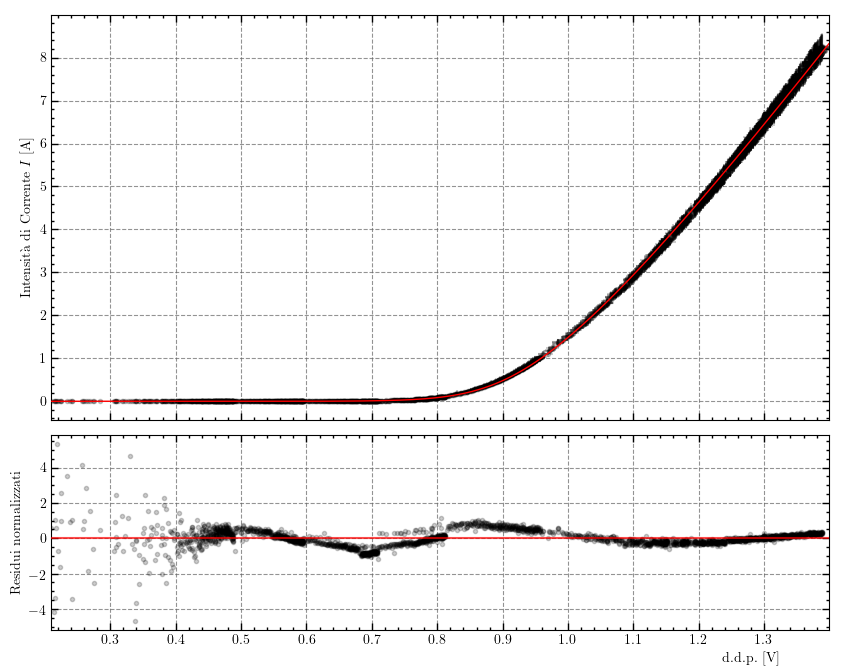
\includegraphics[width=16cm, height= 11cm]
		{100skip_linear}
	\caption{Dati acquisiti e funzione di best-fit \eqref{eq: model}. E' 
	stato rappresentato un punto ogni 100 per comodità di visualizzazione.
	\label{fig: sck_lin}}
\end{figure}

\begin{figure}[!htp]
	\centering 
		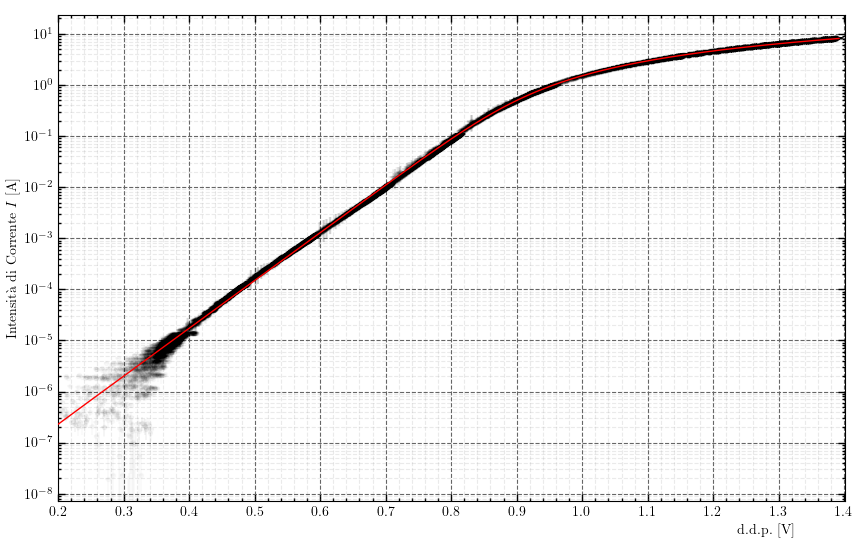
\includegraphics[width=16cm, height= 9.9cm]{10skip_semilog}
	\caption{Dati acquisiti e funzione di best fit \eqref{eq: model} in 
	scala semilogaritmica. A scopo illustrativo sono stati rappresentati anche
	i dati della serie 220k. E' stato disegnato un punto ogni 10 per comodità
	di visualizzazione. \label{fig: sck_log}}
\end{figure}

% Baldini e Fuso dicono sempre di specificare come si è implementato
% il procedimento di fit (numerico/analitico,... con che algoritmo?
% Levenberg-Marquardt, etc). Una volta avevo scritto una bozza su curve_fit e
% Scipy, ma credo sia stata eliminata. O qua o in Appendice B forse dovremmo
% almeno menzionarlo da qualche parte.

%================================================================
%                          Conclusioni
%================================================================
\section{Conclusioni}
Per prima cosa osserviamo dall'analisi appena effettuata, che il
$\chi^2$ risulta minore rispetto al suo valore atteso. Ciò \`e
parzialmente dovuto alla correlazione degli errori sulle misure eseguite
dai due canali d'ingresso. In aggiunta, come si può notare dalla
zona di maggior concentrazione dei punti nel grafico dei residui,
il convertitore analogico-digitale del MCU \`e caratterizzato da una funzione
di risposta non lineare. Questo fattore era stato tenuto in considerazione
all'interno della calibrazione delle porte \verb+ADC0+ e \verb+ADC1+ mediante
l'aggiunta in quadratura di un errore di natura non statistica a quelli stimati
attraverso il fit lineare. Tale operazione ha portato, quindi, ad
un'ulteriore diminuzione del $\chi^2$ all'interno del fit finale.
Ulteriori osservazioni possono essere condotte riguardo alle evidenti analogie
di carattere qualitativo fra la zona di maggior concentrazione dei
campionamenti e la funzione di best fit.
In primo luogo: all'interno del grafico in scala lineare, a correnti alte,
i punti risultano essere disposti pressoch\`e linearmente, in accordo con
l'ipotesi di una componente resistiva interna al diodo. Analogamente, nel
grafico in scala semilogaritmica, i dati assumono un andamento simile a quello
caratteristico della curva di Shockley, ovvero approssimativamente
rettilineo, per poi appiattirsi come un logaritmo al crescere della tensione.
Dunque, possiamo concludere che il fit con il modello \eqref{eq: model} è un
buon fit e, entro i limiti sperimentali, questo risulta in buon accordo con
il comportamento di un diodo reale, per cui non abbiamo motivo di rigettarlo.
Pertanto potremo aspettarci che i parametri stimati dal fit siano significativi 
e che la modellizzazione proposta sia una buona approssimazione del diodo reale 
nelle condizioni di lavoro considerate. Questa modellizzazione, fra l'altro, 
può risultare utile nelle simulazioni numeriche di circuiti con diodi in regimi
impulsati su alte correnti, specialmente ove sia richiesto un dettaglio
sulle cadute di tensione sui singoli componenti. 
%Per tale scopo la legge \eqref{eq: model} \`e confermata essere una buona
%approssimazione del diodo reale entro i limiti sperimentali.
Sebbene questo studio sia concentrato su un unico diodo 1N4007, il metodo
proposto pu\`o essere esteso per qualunque altro tipo di diodo, eventualmente
sostituendo il condensatore con un opportuno circuito stabilizzatore di
corrente o di tensione.

%================================================================
%                        Appendice A
%================================================================
\section{Appendice A: Misurazione delle reristenze $R1$}\label{app: A}

All’interno delle misurazioni delle resistenze, sono stati adottati dei resistori
contrassegnati da valori nominali che spaziano da 0.22 $\Omega$ a 220 $k\Omega$.
Dunque il multimetro digitale non possiede una sensibilità sufficiente ai fini
della stima delle resistenze più basse.\\  
In primo luogo, queste ultime sono state misurate attraverso un metodo basato
sull’uso di un alimentatore regolabile DC ($\Delta V_{\text{max}} = 30 V$;
$I_{\text{max}} = 5 A$). La strategia consiste nel fare scorrere una corrente
continua entro un resistore. La stessa deve essere scelta ponendo attenzione
che la potenza dissipata ($P =R \cdot I^{2}$) non superi la potenza nominale
del resistore onde evitare danneggiamenti del componente per effetto termico.
Nel contempo, la corrente \footnote{La corrente è stata misurata col multimetro,
nonostante il fatto che l’abbiamo scelta a priori, ai fini di ottenere una maggiore precisione}
e la differenza di potenziale ai capi del resistore vengono misurati attraverso
due multimetri digitali. Dunque attraverso la legge di Ohm è stato possibile la
stima delle resistenze in esame, riportate nella tabella sottostante con i relativi errori:

\begin{table}[H]
\begin{center}
    \begin{tabular}{lll}
     \toprule
     $R1$ nom. [$\Omega$] & $R1$ [$\Omega$] \\
     \midrule
     \midrule
     $0.22 \pm 3 \% $     & $0.22 \pm 0.01 $ \\
     $2.2 \pm 5 \% $     & $2.19 \pm 0.03 $ \\
     $22 \pm 5 \% $     & $21.6 \pm 0.2 $ \\
        $220 \pm 5 \% $     & $210.6 \pm 0.8 $ \\
     $2.2\; \rm k \pm 5 \% $ & $2140 \pm 23$ \\
     \bottomrule
    \end{tabular}
    \caption{I valori delle resistenze poste in serie al diodo, riportate in
        valore nominale e misurate con il primo metodo. \label{tab:res}}
\end{center}
\end{table}

Successivamente, è stato adottato un approccio differente. Ai fini di effettuare le medesime
misure, è stato adottato il metodo della misura a quattro terminali (4T), attraverso un ohmetro
specifico. Ai valori misurati sono stati sottratte le letture effettuate in assenza del resistore.
In tal modo, sono stati cancellati gli errori dovuti alle resistenze intrinseche dei fili. Nella
presente tabella sono riportati i risultati conseguiti:

\begin{table}[H]
\begin{center}
    \begin{tabular}{lll}
     \toprule
     $R1$ nom. [$\Omega$] & $R1$ [$\Omega$] \\
     \midrule
     \midrule
     $0.22 \pm 3 \% $     & $0.226 \pm 0.008$ \\
     $2.2 \pm 5 \% $     & $2.212 \pm 0.008$ \\
     $22 \pm 5 \% $     & $21.86 \pm 0.010$ \\
        $220 \pm 5 \% $     & $216.22 \pm 0.07$ \\
     $2.2\; \rm k \pm 5 \% $ & $2202.1 \pm 0.4$ \\
     \bottomrule
    \end{tabular}
    \caption{I valori delle resistenze poste in serie al diodo, riportate in
        valore nominale e misurate con la seconda strategia. \label{tab:res}}
\end{center}
\end{table}

Entrambi i metodi forniscono stime valide delle resistenze adottate. Dunque all’interno
delle analisi successive, sono state adottate le misure conseguite a seguito della
seconda strategia, caratterizzate da maggiore precisione.\\
Le resistenze da 22 $k\Omega$ e 220 $k\Omega$ sono state invece misurate con l’uso
diretto di un multimetro digitale.

%================================================================
%                        Appendice B
%================================================================
\section{Appendice B: Filtraggio Dati}\label{app: B}
%================================
%         Introduzione
%================================
\subsection{Introduzione}
All'interno dell'acquisizione, sono stati raccolti un numero ingente di dati,
suddivisibili in base alla resistenza adottata e dunque facenti riferimento
a zone differenti della curva. A seguito della calibrazione, ci si è quindi
posto il problema di effettuare l'eliminazione degli outliers in modo
indipendente dalla scelta del modello per il fit. Le serie effettuate
variando la resistenza, inoltre, si sovrappongono in alcune zone del
grafico. Dunque è stato necessario eliminare i dati che, non aggiungendo
informazioni utili, andavano a "sporcare" il grafico.
Il sistema di filtraggio di dati implementato
nell'eseguibile si compone di 2 fasi: la prima consiste nell'eliminazione degli
outliers, la seconda dei dati non significativi.
%================================
%         Procedimento
%================================
\subsection{Procedimento}
Supponiamo di avere una serie di dati $(x, y)$ e assumiamo che siano
indipendenti tra loro. Quest'ipotesi non è vera in generale, ma
è tanto più lecita quanto più la correlazione tra le varianze delle misure su
$x$ e $y$ è indipendente dai valori assunti dalle $x$ e $y$ stesse e quanto più
sono numerosi i dati racchiusi entro una deviazione standard lungo $x$ per 
ciascun elemento: in questo caso, infatti, la correlazione viene inclusa nella
varianza lungo $y$.
Supponiamo inoltre che siano note a priori le $\sigma_x ^2 \coloneqq \var{x}$
e che la loro distribuzione di probabilità sia normale (le distribuzioni
delle componenti sono approssimativamente gaussiane per il convertitore
di \verb+Teensy+, perlomeno utilizzando la risoluzione a 12 bit) secondo una 
matrice
di covarianza diagonale nella base $\left\{x, y\right\}$.
In ogni modo, i nostri dati $x$ e $y$ risultano indipendenti e
approssimativamente normali. Dunque le assunzioni risultano giustificate. 
Conseguentemente la densità di probabilità che un punto misurato in $x$ si trovi
a tale ascissa $x_i$, si ricava integrando lungo $y$ a $x$ fissata:
\[
	\ud P = \frac{1}{\sigma_{x_i} \sqrt{2\pi}}
	e^{-\frac{1}{2}{\frac{(x - x_i)^2}{\sigma_{x_i}^2}}} \ud x
.\] 
Dunque, ripetendo più volte la stessa misura, si otterrà la probabilità:
\[
	P\left(\mid x - x_i \mid \leq \frac{\eps}{2} \right) = \eps G_{x_i} 
.\]
dove \[
	G_{x_i} \coloneqq \frac{1}{\sigma_{x_i} \sqrt{2\pi}}
	e^{-\frac{1}{2}{\frac{(x - x_i)^2}{\sigma_{x_i}^2}}}
.\] 
e $\eps > 0$ e $\eps \longrightarrow 0$. Scegliendo allora solo quelle misure $x$ per
cui vale $\mid x - x_i \mid \leq \frac{\eps}{2}$, queste saranno in numero
tendente a:
\[
	N_i \coloneqq N_{\text{tot}} \frac{G_{x_i}}{\sum_j G_{x_j}} =
		N_{\text{tot}} w_i
.\] 
che definisce implicitamente i pesi $w_i$ con cui si mediano le distribuzioni
di probabilità gaussiane $G_{x_i}$.
Allora, posto:
\[
	G_{y_i} \coloneqq \frac{1}{\sigma_{y_i} \sqrt{2\pi}}
	e^{-\frac{1}{2}{\frac{(\mu_y - y_i)^2}{\sigma_{y_i}^2}}}
.\] 
Per il principio di massima verosimiglianza siamo quindi interessati a
massimizzare la quantità:% è una roba matematica, non è fisica
\[
	\like = \prod_{i=1}^{n} \prod_{j=1}^{N_i} G_{y_i} = 
	\prod_{i=1}^{n} G_{y_i}^{N_i}
.\] 
Per la monotonia del logaritmo il problema equivale a massimizzare: 
\[
	\ln{\like} = \sum_{i=1}^{n}\ln{G_{y_i}}^{N_{\text{tot}}w_i} = 
	\frac{N_{\text{tot}}} {\sum_{j=1}^{n} G_{x_j}} 
	\sum_{i=1}^{n} G_{x_i} \ln{G_{y_i}}
.\] 
Per cui, a meno di costanti risulta:
\begin{equation}\label{eq: likeconst}
	\ln{\like} - \text{const.} \propto \sum_{i=1}^{n} -G_{x_i} \ln{\sigma_y}
	- \frac{1}{2} G_{x_i} \left( \frac{y_i - \mu_y}{\sigma_y} \right)^2
\end{equation}
Imponendo la condizione di stazionarietà rispetto a $\mu_y$ si ottiene dunque:
\begin{equation}\label{eq: muy}
	\mu_y = \sum_{i=1}^{n} y_i w_i 
\end{equation} 
Una volta sostituito in \eqref{eq: likeconst} quanto appena trovato per $\mu_y$
e imponendo la stessa condizione di stazionarietà rispetto a $\sigma_y$ si ha:
\begin{equation}\label{eq: sigmay}
	\sigma_y^2 = \sum_{i=1}^{n} (y_i - \mu_y)^2 w_i
\end{equation}
Infine è possibile ricavare la varianza di $\mu_y$ dalla definizione di valore
di aspettazione, riconducendola più volte a integrali di gaussiane di altezze
e ampiezze diverse:
\begin{align} \label{aln: varmuy}
%	\var{\mu_y} &= \sum_{i=1}^{n} w_i^2 \sigma_y^2 + 
%	\left(\frac{y_i}{\sum_{j=1}^{n} w_j}  \right)^2 \frac{
%	\frac{e^{-\frac{(x-x_i)^2}{3 \sigma_x^2}}} {\sigma_x \sqrt{6 \pi} } +
%	\frac{e^{-3\frac{(x-x_i)^2}{4 \sigma_x^2}}} {\sigma_x \sqrt{\pi} } +
%	\frac{e^{-\frac{(x-x_i)^2}{\sigma_x^2}}} {\sigma_x \sqrt{2 \pi}}
%	} {\sqrt{2 \pi}} =\\ 
	\var{\mu_y} &= \sum_{i=1}^{n} w_i^2 \sigma_y^2 + 
	\left(\frac{y_i}{\sum_{j=1}^{n} w_j} \right)^2 \frac{
	e^{-\frac{(x-x_i)^2}{3 \sigma_{x_i}^2}} +  
	\sqrt{3} \left( e^{-\frac{(x-x_i)^2}{\sigma_{x_i}^2}} -
	\sqrt{2} e^{-3 \frac{(x-x_i)^2}{4 \sigma_{x_i}^2}} \right)
	} {2 \sqrt{3}\pi \sigma_{x_i}^2} 
\end{align}
Riassumendo:\\
Nella \eqref{eq: muy} prendiamo una media dei campionamenti intorno ad un'
ascissa $x$ in esame, pesata sulla distanza che gli $x_i$ hanno da questa; 
intuitivamente lo interpretiamo come se stessimo applicando un 
\emph{blur a kernel gaussiano} ai punti acquisiti.
Effettivamente quello che stiamo facendo non è molto diverso da KDE monovariante,
dove però scaliamo secondo il valore delle $y$.
Lo stesso ragionamento vale per $\sigma_y^2$, si ha una stima della varianza
dei dati la variare di $y$, pesata sulla distanza dai valori studiati. Dunque
$\mu_y \pm \sigma_y$ ci dà una descrizione della distribuzione dei nostri dati.

%================================
%           Var(muy)
%================================
\subsection{$\var{\mu_y}$}
Mentre $\sigma_y$ rappresenta la distribuzione dei dati intorno al valor medio 
$\mu_y$, $\var{\mu_y}$ ci indica l’incertezza sulla miglior stima di $y$.
Questo è utile per determinare la convergenza della stima in funzione dei dati
acquisiti. Infatti tanto più è elevata la densità dei dati, rispetto alla
deviazione standard $\sigma_x$, tanto più la stima del valore centrale risulta
precisa.
Graficamente la banda di confidenza è più ristretta dove si concentrano i dati.
Viceversa, la stessa tende ad allargarsi dove i dati sono sparsi, i.e. a
distanze paragonabili a $\sigma_x$. Numericamente, si vede dalla seconda somma
nell'espressione \eqref{aln: varmuy} che la stima del valore centrale è
statisticamente significativa solo quando si media su un intervallo campionato
con almeno qualche punto ogni deviazione $\sigma_x$: altrimenti $\sigma_y \to 0$
indicando così assenza di dati, mentre $\var{\mu_y}$ tende a $+\infty$ come
$\sim e^{x^2}$, indice della stessa insufficienza di dati al fine di stabilire
con precisione significativa il valore di $\mu_y$.
\begin{figure}[!htb]
	\centering 
 		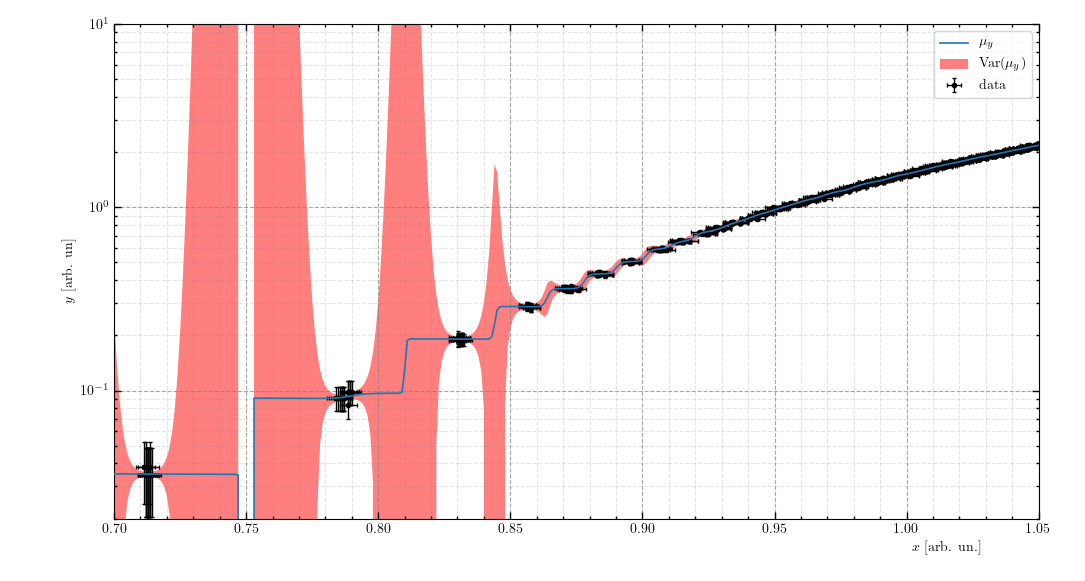
\includegraphics[scale=0.55]{./varmuy.png}
 	\caption{La media $\mu_y$ è rappresentata dalla linea blu, mentre
	l'area in rosso indica il valore di $\var{\mu_y}$ al variare dei
	dati (in nero) lungo $x$. \label{fig: varmuy}}
\end{figure}
Nel caso opposto, in cui i dati sono "densi" (in confronto alle $\sigma_x$)
la seconda somma, per quanto computazionalmente intensiva, numericamente
sembrerebbe piccola in confronto alla prima: in realtà non lo è, ma
soprattutto questa non può essere trascurata, poiché è proprio la quantità
che descrive la dipendenza dalla densità stessa e dunque la caratteristica
convergenza/divergenza della precisione sulla stima centrale fornita.

%================================
%        Filtro outliers
%================================
\subsection{Filtro outliers}
La parte più semplice nel filtraggio dati consiste nello scartare tutti quei
punti che distano da $\mu_y$ più di una soglia arbitraria $k$ di deviazioni
standard $\sigma_y$ (nel nostro caso è stato scelto $k = 2$, non critico,
trovato dopo una serie di prove). A differenza del classico metodo basato
sulla distanza dalla curva/modello di best fit, per il nostro criterio essa
è ininfluente. Questo risulta particolarmente utile in simili situazioni di
verifica del modello in quanto una selezione basata su un preliminare fit
risulterebbe influenzata dalla scelta della funzione in questione e
eliminerebbe tutti i dati che non risultano compatibili con essa.
%indipendentemente dal modello di fit vale $|y_i - \mu_y| \geq k\sigma_y$.

%================================
%  Filtro dati non significativi
%================================
\subsection{Filtro dati non significativi}
Supponiamo di avere 2 set di dati fatti con diverse resistenze, il primo $(A)$
con una resistenza bassa, il secondo $(B)$ con una alta: Il primo set esplorerà
la regione ad alta corrente, mentre il secondo la regione di basse correnti.
In generale i dati del primo si sovrapporranno anche nelle zone basse esplorate
dal secondo, però senza aggiungere sostanziali informazioni rispetto a quanto
farebbe il secondo.
%Il nostro obiettivo è dunque eliminare questi dati meno significativi.
Esponiamo dunque il criterio sviluppato per ridurre l'influenza di questi
punti meno significativi sulla ricerca dei parametri di best-fit e sulla
rappresentazione finale dei dati.\\
Per capire se in un certo punto i dati di $A$ sono significativi, calcoliamo
la misura di significatività che abbiamo sviluppato in \eqref{aln: varmuy}$:
\var{\mu_y}$ di $A$ e di $B$. Perciò se $\var{\mu_y}$ di $A$ è maggiore di 
$q\var{\mu_y}$ di $B$, con $q$ arbitrario (nell'esperienza è stato scelto
$q = 3$), questo indica che i dati di $A$
ci stanno dando "poca" informazione rispetto a quelli di $B$. A questo punto
è sufficiente controllare tutti i punti scorrendo su tutte le combinazioni
di set per eliminare i dati non significativi, che rendono meno
immediata l'interpretazione del grafico. Questo è ben visibile in scala
logaritmica sulle $y$, dove i punti con grandi incertezze o varianze tendono
a disperdersi rapidamente.
L’algoritmo è computazionalmente intensivo e richiede una corretta gestione
della memoria per evitare bolle di allocazione. Dunque è stato implementato
in \verb'C++' per praticità e richiamato all’interno degli script (per dettagli si 
rimanda ai 
\href{https://github.com/LucaCiucci/relaz_seme/tree/master/Cartella_fit/filter_src}{sorgenti}).
Nelle figure di esempio sono mostrati i dati selezionati dall’algoritmo
(in nero) ed i dati scartati (in arancio). 

\begin{figure}[!htbp]% per questi non ci dovrebbero essere problemi, basta che non vanno in B
\centering
\begin{subfigure}{.5\textwidth}
	\centering 
 		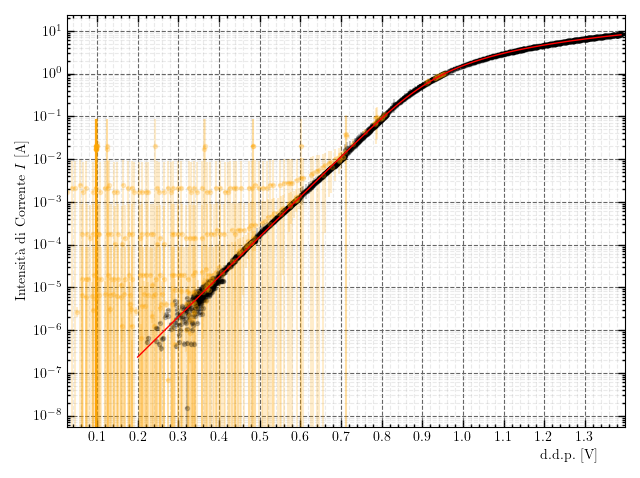
\includegraphics[scale=0.5]{./nofilter.png}
		\caption{\label{fig: nofilter}}	
\end{subfigure}%
\begin{subfigure}{.5\textwidth}
	\centering 
 		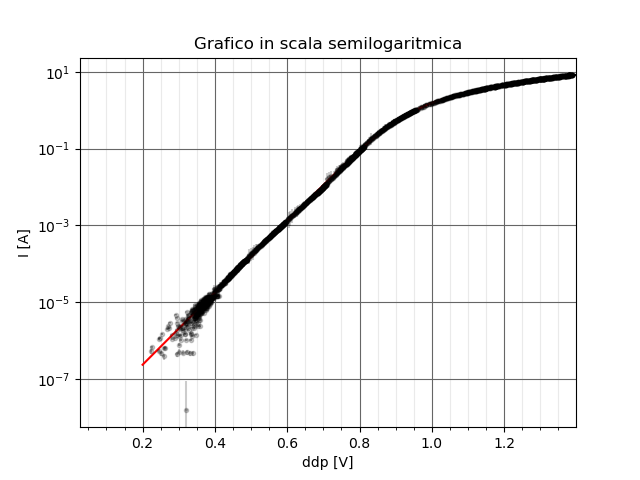
\includegraphics[scale=0.5]{./filtered.png}
 	\caption{\label{fig: filtered}}
\end{subfigure}
\caption{Grafici in scala semilogaritmica prima (\ref{fig: nofilter}) e dopo 
(\ref{fig: filtered}) del filtraggio dati. I dati scartati sono stati
evidenziati in arancio. Per praticità è stato rappresentato un centesimo
dei dati raccolti}
\end{figure}
\`E infine mostrato il confronto dei grafici delle $\var{\mu_y}$
tra due set successivi.
\begin{figure}[!h]
	\centering 
 		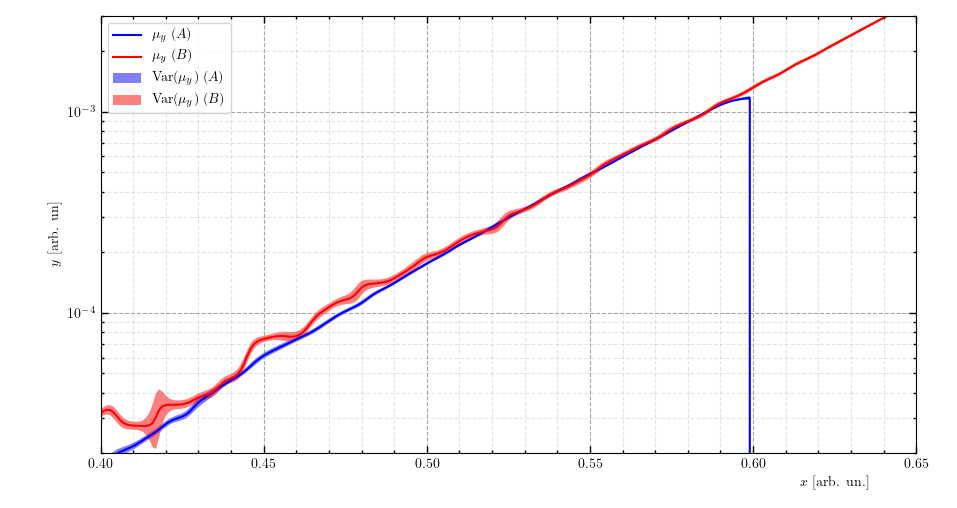
\includegraphics[scale=0.65]{comparison.png}
 	\caption{Confronto dei grafici delle $\var{\mu_y}$ su due set di
	dati consecutivi. \label{fig: comparison}}
\end{figure}

%================================================================
%                        Appendice C
%================================================================
\section{Appendice C: Metodo di fit}\label{app: C}
La differenza di potenziale $\Delta$V in funzione della corrente $I$ che scorre 
all’interno del diodo può essere espressa attraverso la legge
\eqref{eq: model}. Potremo, dunque, essere tentati ad adottare tale formula
ai fini di un fit numerico. 
Tuttavia tale operazione provocherebbe il fallimento del fit a causa dei valori 
negativi o nulli che debitamente si riscontreranno all’interno del logaritmo. 
E’ stato dunque necessario adottare un algoritmo alternativo, basato sul 
metodo di Newton\cite{tesi}. Esso ci consentirà di ricostruire numericamente 
la funzione inversa della legge \eqref{eq: model}.
Illustriamo in breve il metodo di Newton. Sia data una funzione $f(x)$ continua e di classe $C^{2}$
entro un intervallo di definizione connesso (con $f’(x)$ limitata e 
diversa da $0$ per ciascuna $x$ appartenente al dominio) ed una $v$ tale che
$f(v) = 0$. Sviluppando al prim’ordine $f$ in un intorno di $v$, otterremo:
\begin{equation}
f(x) = f(v) + f{'}(v) + {\frac{1}{2}} {f{''}(X)} \cdot  {( x - v)^2} = 0
\end{equation}
ove $X$ è un numero reale compreso fra $v$ ed $x$. Nel caso in cui il $(x-v)^2 
$risultasse prossimo a zero:
\begin{equation}
x \simeq v   -  {\frac {f(v)}{f’(v)}}
\end{equation}
L’unica limitazione nell'adottare tale scrittura è che necessitiamo di $v$ 
molto vicino a $x$ incognito. Tuttavia, nel caso in cui la funzione $f$ risultasse 
sufficientemente maneggevole, potremo partire da un valore generico del dominio 
e riscontrare con buona approssimazione la radice in un tempo finito 
relativamente breve. Per effettuare ciò, è necessaria la serie ricorsiva:
\begin{equation}
\begin{cases}
x[0] = a \\ x[N+1] = x[N] - \frac {f(x[N])} {f’(x[N])}
\end{cases}
\end{equation}
ove $a$ è un generico valore appartenente al dominio di definizione. In pratica, 
per ogni iterazione tale serie valuta $f(x[i])$ e cerca la retta tangente in tale 
punto alla funzione:
\begin{equation}
y = f(x[i]) + f’(x[i]) \cdot (x-x[i])
\end{equation}
 Dopodiché cerca il punto $x$ per il quale $y = 0$:
\begin{equation}
x = x[i+1] = x[i] - \frac{f(x[i])}{f’([i])}
\end{equation}
E viene conseguentemente valutato il valore $f(x[i+1])$ ed il procedimento viene 
ripetuto per un dato numero di iterazioni. 
\begin{figure}[!htbp]
	\centering 
 		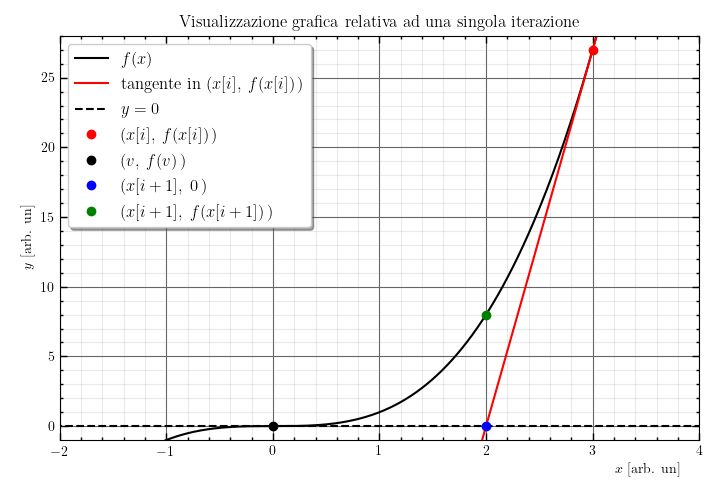
\includegraphics[scale=0.8]{tang.png}
	\caption{Visualizzazione grafica di cosa implica un’iterazione della 
	serie ricorsiva ($f(x) = x^3$ in questo esempio)\label{fig: tang}}
\end{figure}
Se la funzione è monotona e la serie converge ad un valore, tale sarà $v$, 
essendo l’unico punto fisso della serie:
\begin{equation}
 a = a -  \frac{f(a)}{f'(a)} \to f(a) = 0 \; \land \; v = a
\end{equation}
essendo $v$ l’unico punto in cui si annulla la funzione per definizione.
Ritornando al diodo, esso può essere interpretato quale un diodo ideale ed una 
resistenza in serie, collegati ad un generatore di differenza di potenziale. 
Quindi, per la legge delle maglie:
\begin{equation}
\Delta V_{\text{ingresso}} = \Delta V_{\text{diodo}} + \Delta 
V_{\text{resistenza}} = \Delta V_{\text{diodo}} + R \cdot I
\end{equation}
ove $I$ è la corrente che scorre all’interno del diodo in quel determinato 
istante. Notoriamente, tale scrittura si può porre nella seguente forma ai 
fini di definire la retta di carico del diodo:
\begin{equation}
\Delta V_{\text{diodo}} = \Delta V_{\text{ingresso}} - R \cdot I
\end{equation}
Il punto di intersezione di tale retta con l’equazione di Shockley per il 
diodo rappresenta il punto di lavoro $(v, i)$ del diodo:
\begin{equation}
i = I_0 \cdot ( e^{\frac {\Delta V_{\text{ingresso}} - R \cdot i}{\eta V_T} } - 
1) = I_0 \cdot (e^{\frac{v} {\eta V_T}} -1) =  \frac{\Delta V_{\text{ingresso}} 
- v}{R}
\end{equation}
Tale $i$ dovrà necessariamente corrispondere alla corrente di lavoro in virtù 
dell’equazione di Shockley. Dunque definendo la funzione $g(x)$ come segue:
\begin{equation}\label{eq: invsck}
g(x) = I_0 \cdot ( e^{\frac{x}{\eta V_T}} - 1)  - \frac {\Delta 
V_{\text{ingresso}} - x}{R}
\end{equation}
è possibile adottare il metodo di Newton al fine di riscontrare la radice $v$
ed individuare così la corrente di lavoro. 
Dunque si potrà effettuare un fit della corrente in funzione della tensione ai 
capi del diodo reale attraverso una legge che per un determinato valore della 
tensione ($\Delta V_{\text{ingresso}}$) ed un dato numero di iterazioni (ne 
sono sufficienti poche nel nostro caso ai fini di ottenere un’approssimazione 
adeguata), riesce ad individuare la radice $v$ nelle modalità previamente 
descritte. Attraverso la stessa, sarà quindi possibile individuare la corrente 
di lavoro del diodo per la suddetta $\Delta V_{\text{ingresso}}$. 
\`E immediato comprendere che fare un fit con questa legge risulta essere 
equivalente a fare un fit con la legge \eqref{eq: model}, con minori complicazioni 
computazionali. Verifichiamo graficamente che per dei generici valori della 
corrente i due metodi danno risultati sostanzialmente equivalenti (adottiamo i 
parametri stimati dal fit). I grafici relativi alla convergenza di $I$ e di $v$ 
anche a seguito di sole 20 iterazioni:
\begin{figure}[H]
	\centering 
	\def\svgwidth{\columnwidth}
		\scalebox{0.75}{\includesvg{Iter}}
\end{figure}
\begin{figure}[H]
	\centering 
		\scalebox{0.75}{\includesvg{vter}}
\end{figure}
Tali grafici evidenziano che, come era da aspettarsi, la legge adottata per il 
fit risulta essere l’inversa numerica della legge \eqref{eq: model}. La serie,
inoltre, risulta convergere molto rapidamente ai valori attesi e quindi sono 
effettivamente sufficienti solo 20 iterazioni per una buona precisione.
All’interno della funzione di fit, è stato infine introdotto un offset quale
parametro libero per ovviare errori di zero dovuti agli assorbimenti di ADC
in Teensy 3.2.

\subsection*{Nota sull'implementazione}
Per determinare i parametri ottimali e le rispettive covarianze si \`e
implementato in \verb+Python+ un algoritmo di fit basato sui minimi quadrati
mediante la funzione \emph{curve\_fit} della libreria \texttt{Scipy}\cite{scipy}
Per tutti i fit su campionamenti digitali di \verb+Teensy+ si è imposto
$\rm{abs\_sigma} =$ False, in quanto la sorgente principale d'incertezza
sulle misure risulta non statistica/non determinata.
%per cui non sarebbe giustificato assumere come errore il valore convenzionale
%$\sigma = \pm 1$ [digit] effettivamente si esegue un fit dei minimi quadrati.

%================================================================
%                            END
%================================================================
\medskip
\bibliographystyle{IEEEtrandoi}
\bibliography{refs}
\end{document}
